% !TeX root = ../main.tex

\ustcsetup{
  cite-style = authoryear,
}
 

\chapter{绪论}

\section{引言}

地震是一种自然现象,地震学是一门研究地震的学科。
地震学依赖于观测技术,其完备的数学物理基础决定了它在自然科学研究中扮演着重要的作用。
地震如一盏明灯,照亮地下发生的一切\citep{陈颙2017}。
地震学家利用地震仪记录振动信号,研究地球内部结构、地震震源特性以及动力学过程等,其基本数学语言可表达为:
\begin{equation}
  u(t)=s(t)*g(t)*i(t)
\end{equation}
其中,$u(t)$是地震记录即振动信号,$s(t)$是震源项,$g(t)$是结构项,$i(t)$是地震仪器响应项。

地震信号种类很多,例如天然地震、火山喷发、海浪与飓风、人工爆破、油气开采以及各种人类活动等。
地震信号的能量差异很大,大到板块俯冲带的巨型地震(例如,311东北大地震\footnote{2011年3月11日,日本宫城县牡鹿半岛东南偏东130千米的西北太平洋海域处发生了矩震级9.0的地震}),
其矩震级$M_w$可达到9;
小到油气开采时地下微裂缝的破裂,其矩震级可以小于0。

地震学的发展离不开观测手段的进步,从传统的地震仪,发展到现在的旋转地震仪、智能节点式地震仪与
DAS(Distributed Acoustic Sensing Technique,分布式声学信号传感技术)等。
观测手段的进步引导着研究方法的发展,近些年基于机器学习、深度学习、大数据与云计算平台,
地震学家正拥有着前所未有的计算资源与观测密度,发现并监测着我们脚下的一举一动,地震学正迎来新的机遇与挑战。

地震学的研究方向众多,本文主要聚焦于地震震源参数与背景噪声干涉的研究。
准确的地震震源参数是地震震源研究与地震灾害评估的关键,利用不同相位的到时信息与波形信息,
我们能够反演地震发生的位置、震级、时刻与震源机制解。
本文利用基于贝叶斯采样的蒙特卡洛方法,评估地震双力偶模型与矩张量模型参数中的不确定性,
并将其应用到2021年中国云南漾濞地震与2008年美国Mt. Carmel地震反演中。
背景噪声干涉技术的出现,极大地促进了地震成像与监测研究的进步。
噪声作为一种被动源,不依赖天然地震事件发生的位置,通过互相关运算获得经验格林函数即可应用到地震学的各个方面。
快速的互相关计算是背景噪声干涉技术应用的关键,本文基于Julia编程语言利用多进程与多线程的并行技术,
设计并编写了快速互相关计算的框架。
通过提取经验格林函数中面波的频散信息,我们可以对地下速度结构进行成像研究。
结合高密度的DAS观测手段,背景噪声干涉正在为城市等极端地区提供地震成像研究的可能。
本文利用DAS记录的背景噪声,进行了城市地区地下速度成像的初步研究,并探讨了其中存在的问题与挑战。

% 速度变化监测是背景噪声应用的另一主要方向,其通过研究长时间记录的经验格林函数尾波部分波形与相位的变化,获得相应的结构与速度变化。
% 在区域尺度,其能获得地下速度的变化;在实验室岩石破裂尺度,能够检测微破裂位置,该方法正成为无损检测研究的新领域。
% 本文首先通过数值模拟实验,验证尾波干涉速度变化理论,并定位介质散射点的变化位置,
% 并将背景噪声技术应用于云南大银甸水库附近波速变化的研究。




\section{震源参数研究进展}

准确的震源参数,例如震级、震源位置与震源机制,是地震震源研究的重要课题。
快速准确的震源参数评估,对灾害评估和破坏性地震后的救援工作至关重要。
更好地理解诸如板块运动、火山喷发、海底滑坡与冰川破裂过程等自然现象,离不开对震源参数的准确反演。
空间大地测量技术(例如,全球导航卫星系统与干涉合成孔径雷达)通过对地表静态位移的研究,
能够很好的约束大地震的震源参数\citep{Zha2011,Bathke2013,Vasyura-Bathke2020}。
近些年,一些由非常规油气开发与山体滑坡引起的中小型诱发地震,引起了公众的高度关注\citep{Ellsworth2013,Lei2017,Ruiz-Barajas2017,Zhao2020}。
小地震通常只能引起很小的地表变形,所以很难通过空间大地测量的方法反演地震震源信息。
利用地震仪记录的震动信号,地震学家可以实时反演震源参数,从微地震到巨型地震都很适用。

伴随着震源理论的发展与计算机运算能力的进步,地震学家们先后开发出一系列地震参数反演程序与软件。
多种地震记录信息被应用到震源参数反演中,例如利用极性\citep{Hardebeck2002}、
P波与S波振幅比\citep{Reasenberg1985,Hardebeck2003}、波形信息\citep{Dziewonski1981,Dreger1993}与
多种信息联合反演\citep{Li2011,Tan2018}等。
例如,HASH\citep{Hardebeck2002,Hardebeck2003}程序利用P波和S波极性与P波与S波振幅比的信息,进行震源机制反演。
该算法能够同时考虑地震位置、相位极性与速度模型的误差,并提供了一个对反演结果的评价标准。
全球矩心矩张量项目\citep{Dziewonski1981}与W-phase项目\citep{Kanamori1993}通过拟合
长周期(几十到几百秒)的波形,被广泛应用到中强地震震源参数反演中。
其能够反演地震发生时刻、位置、震级、持续时间、震源机制与矩张量等信息。
但是因为利用长周期波形进行拟合,这些方法往往对地震深度的约束较差。

为了提高对地震深度信息的约束,Cut-And-Paste(CAP)的方法\citep{Zhao1994,Zhu1996}
使用区域地震台网记录的短周期(几秒到十几秒)波形反演双力偶模型的震源机制。
该方法将地震波分成$Pnl$波与面波部分,并且考虑到速度模型的不准确性,
其允许时间窗口在不同相位之间移动。
CAP的方法被广泛应用到区域地震震源机制的研究中\citep{DAmico2011,Ross2015,Zhu2016,Tang2018,Li2020},
并且发展出许多变种方法\citep{Chen2015,Bai2020a}。
近些年有学者提出了广义的CAP方法\citep{Zhu2013},gCAP(generalized Cut-And-Paste),
其能够反演矩张量地震模型的震源机制。


\section{背景噪声研究进展}

在20世纪,地震学的研究主要聚焦在地震事件,利用地震波的多种信息获得地下结构等信息,对地震源的研究帮助人类更好地认识地震危害。
最近20年间,人们发现地震仪记录上非常微弱的振动信号蕴含着丰富的地下信息,尽管产生这些信号的源在不停的变化,我们将其成为背景噪声(ambient noise),如图~\ref{fig:eg-noise}。
尽管地震学家们很早就意识到,海洋潮流、风暴与微震等信号,会在地震记录上显现出来,但很难去量化研究这些信号的潜在作用。
最早利用背景噪声信号研究地下结构的信息,可以追溯到Aki在1957年的工作\citep{aki1957space},其利用台阵记录的背景噪声信息进行空间自相关运算,成功获取了台阵下方的速度结构信息。
在数据处理时,最核心的部分是估计噪声记录里的相关性,其也被认为是两个台站之间的脉冲地震响应,其基本假设是噪声源均匀分布,噪声场充分干涉。
虽然地球上的背景噪声很少能完全满足上面苛刻的条件,但波的神奇之处在于它具有时间可逆性和空间互易性,这使得从背景噪声中提取相关性重建两点之间的脉冲响应成为可能。

21世纪前后,物理学家首先对太阳表面的热噪声信号进行相关性分析,发现随机噪声的互相关运算近似于它们之间的格林函数~\citep{woodard1997implications}。
Lobkis和Weaver~\citep{weaver2001ultrasonics}在实验室声学实验中证实了上述观点,并利用多模态叠加的原理给出了数学物理证明,证明的前提要求波场是完全随机的,且记录时间充分长。
Snieder~\citep{snieder2004extracting}从稳相场(stationary phase)理论出发,证明了台站周围的散射体分布均匀就可以满足上述定理。
Campillo和Paul~\citep{campillo2003long}将其应用在区域尺度研究,并成功从两个台站的地震尾波信号中提取出Rayleigh波和Love波信号。
尾波信号的研究成功后,地震学家开始尝试利用远距离台站噪音记录的长期互相关结果,来恢复两个台站之间的格林函数。
Shapiro和Campillo再次成功从背景噪声中获得了经验格林函数的信号,并在随后的研究中提取了经验格林函数中频散信息,对美国加州地区进行了高分辨率的速度成像,这也是第一个背景噪声面波群速度成像研究~\citep{shapiro2005high}。
Yao等人利用背景噪声提取出面波相速度频散曲线,这也是第一个背景噪声相速度成像的研究~\citep{yao2006surface}。
从此背景噪声的系统性研究工作逐渐开展起来。

事实上,地球上的噪声源多数分布在地球表面,例如海洋风暴和人类活动等,这意味着沿着地表传播的面波将会成为背景噪声中的主要成分,尽管有些研究也能提取出体波信号。
对面波信号进行频散测量可以帮助我们获得地下的速度结构信息。
在不同的日期重复测量,可以实现对研究区域的动态监测,例如测量地震速度的时间变化。
除此之外,利用背景噪声研究地下衰减结构,进行强地面运动信号的恢复,提取体波信号,矫正地震仪器(例如海底OBS)的时钟偏差,提高地震定位经度,研究噪声源分布及其物理特性,以及利用背景噪声进行伴随场成像等,都是背景噪声的研究领域。
背景噪声拥有着广阔的应用前景,包括监测地下工业活动,探测火山爆发、滑坡和地震等自然灾害发生前的微小变化。
现代地震台网记录着大量的连续噪声数据,计算能力的不断提升,
在使用新型传感器(如大型节点阵列、光纤DAS、旋转地震仪)进行观测的时代,背景噪声地震学的应用前景广阔。


\begin{figure}[h]
  \centering
  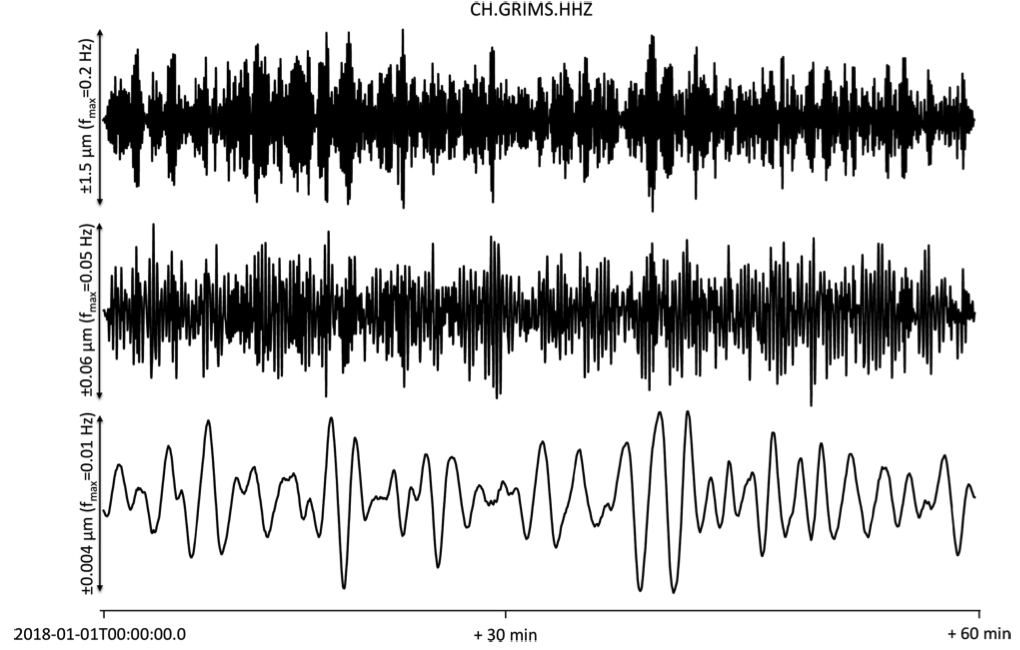
\includegraphics[width=0.9\textwidth]{noise/eg-noise.jpg}
  \caption{背景噪声示例图}
  \label{fig:eg-noise}
  \note{注:瑞士阿尔卑斯山隧道系统内海拔1746米的GRIMS站的垂直分量上记录,低通滤波0.2Hz(上),低通滤波0.05Hz(中),低通滤波0.01Hz(下);图片引自\citep{nakata2019seismic}}
\end{figure}







\section{论文结构安排}

本论文主要分为两部分,震源参数不确定评估与背景噪声干涉成像,具体安排如下。
\begin{enumerate}
  \item 震源参数反演部分:我们首先介绍震源理论,从运动方程出发,推导了位错源模型与体积源模型的震源表达式,并介绍了大中小不同地震的震源模型,然后介绍地震矩张量的分解与可视化;基于贝叶斯蒙特卡洛,我们提出了MCMTpy的方法用于反演震源参数,并将新方法应用到两次地震的研究中,最后讨论了新方法的优点与局限性。
  \item 背景噪声干涉部分:我们首先介绍了三种背景噪声干涉理论,然后介绍了我们进行高性能互相关运算的框架;在介绍背景噪声成像研究之前,我们首先介绍了DAS传感技术,然后介绍我们在2020年北京白家疃DAS观测实验的结果,比较了背景噪声频散成像与主动源频散成像的结果,并对其中存在的问题进行讨论。
  \item 对整篇论文进行总结与讨论,并对未来的研究方向进行展望。
\end{enumerate}









% \subsubsection{三级节标题}

% \paragraph{四级节标题}

% \subparagraph{五级节标题}

% (以下简称《撰写手册》)和
% 《\href{https://www.teach.ustc.edu.cn/notice/notice-teaching/11530.html}


% Lorem
% \footnote{Ut enim ad}
